\subsection{Sequence Diagram}

In the following we describe the sequence diagrams of the main features of the application. 
The sequence diagrams are used to illustrate the interactions between the objects in the system and how they collaborate to achieve a specific functionality. 
The diagrams are presented in a simplified format, focusing on the key interactions and omitting some of the lower-level details for clarity.

%%%%%%%%%%%%%%%%%%%%%%%%%%%%%%%%%%%%%%%%%%%%%%%
\subsubsection{Login}
\begin{figure}[H]
    \centering
    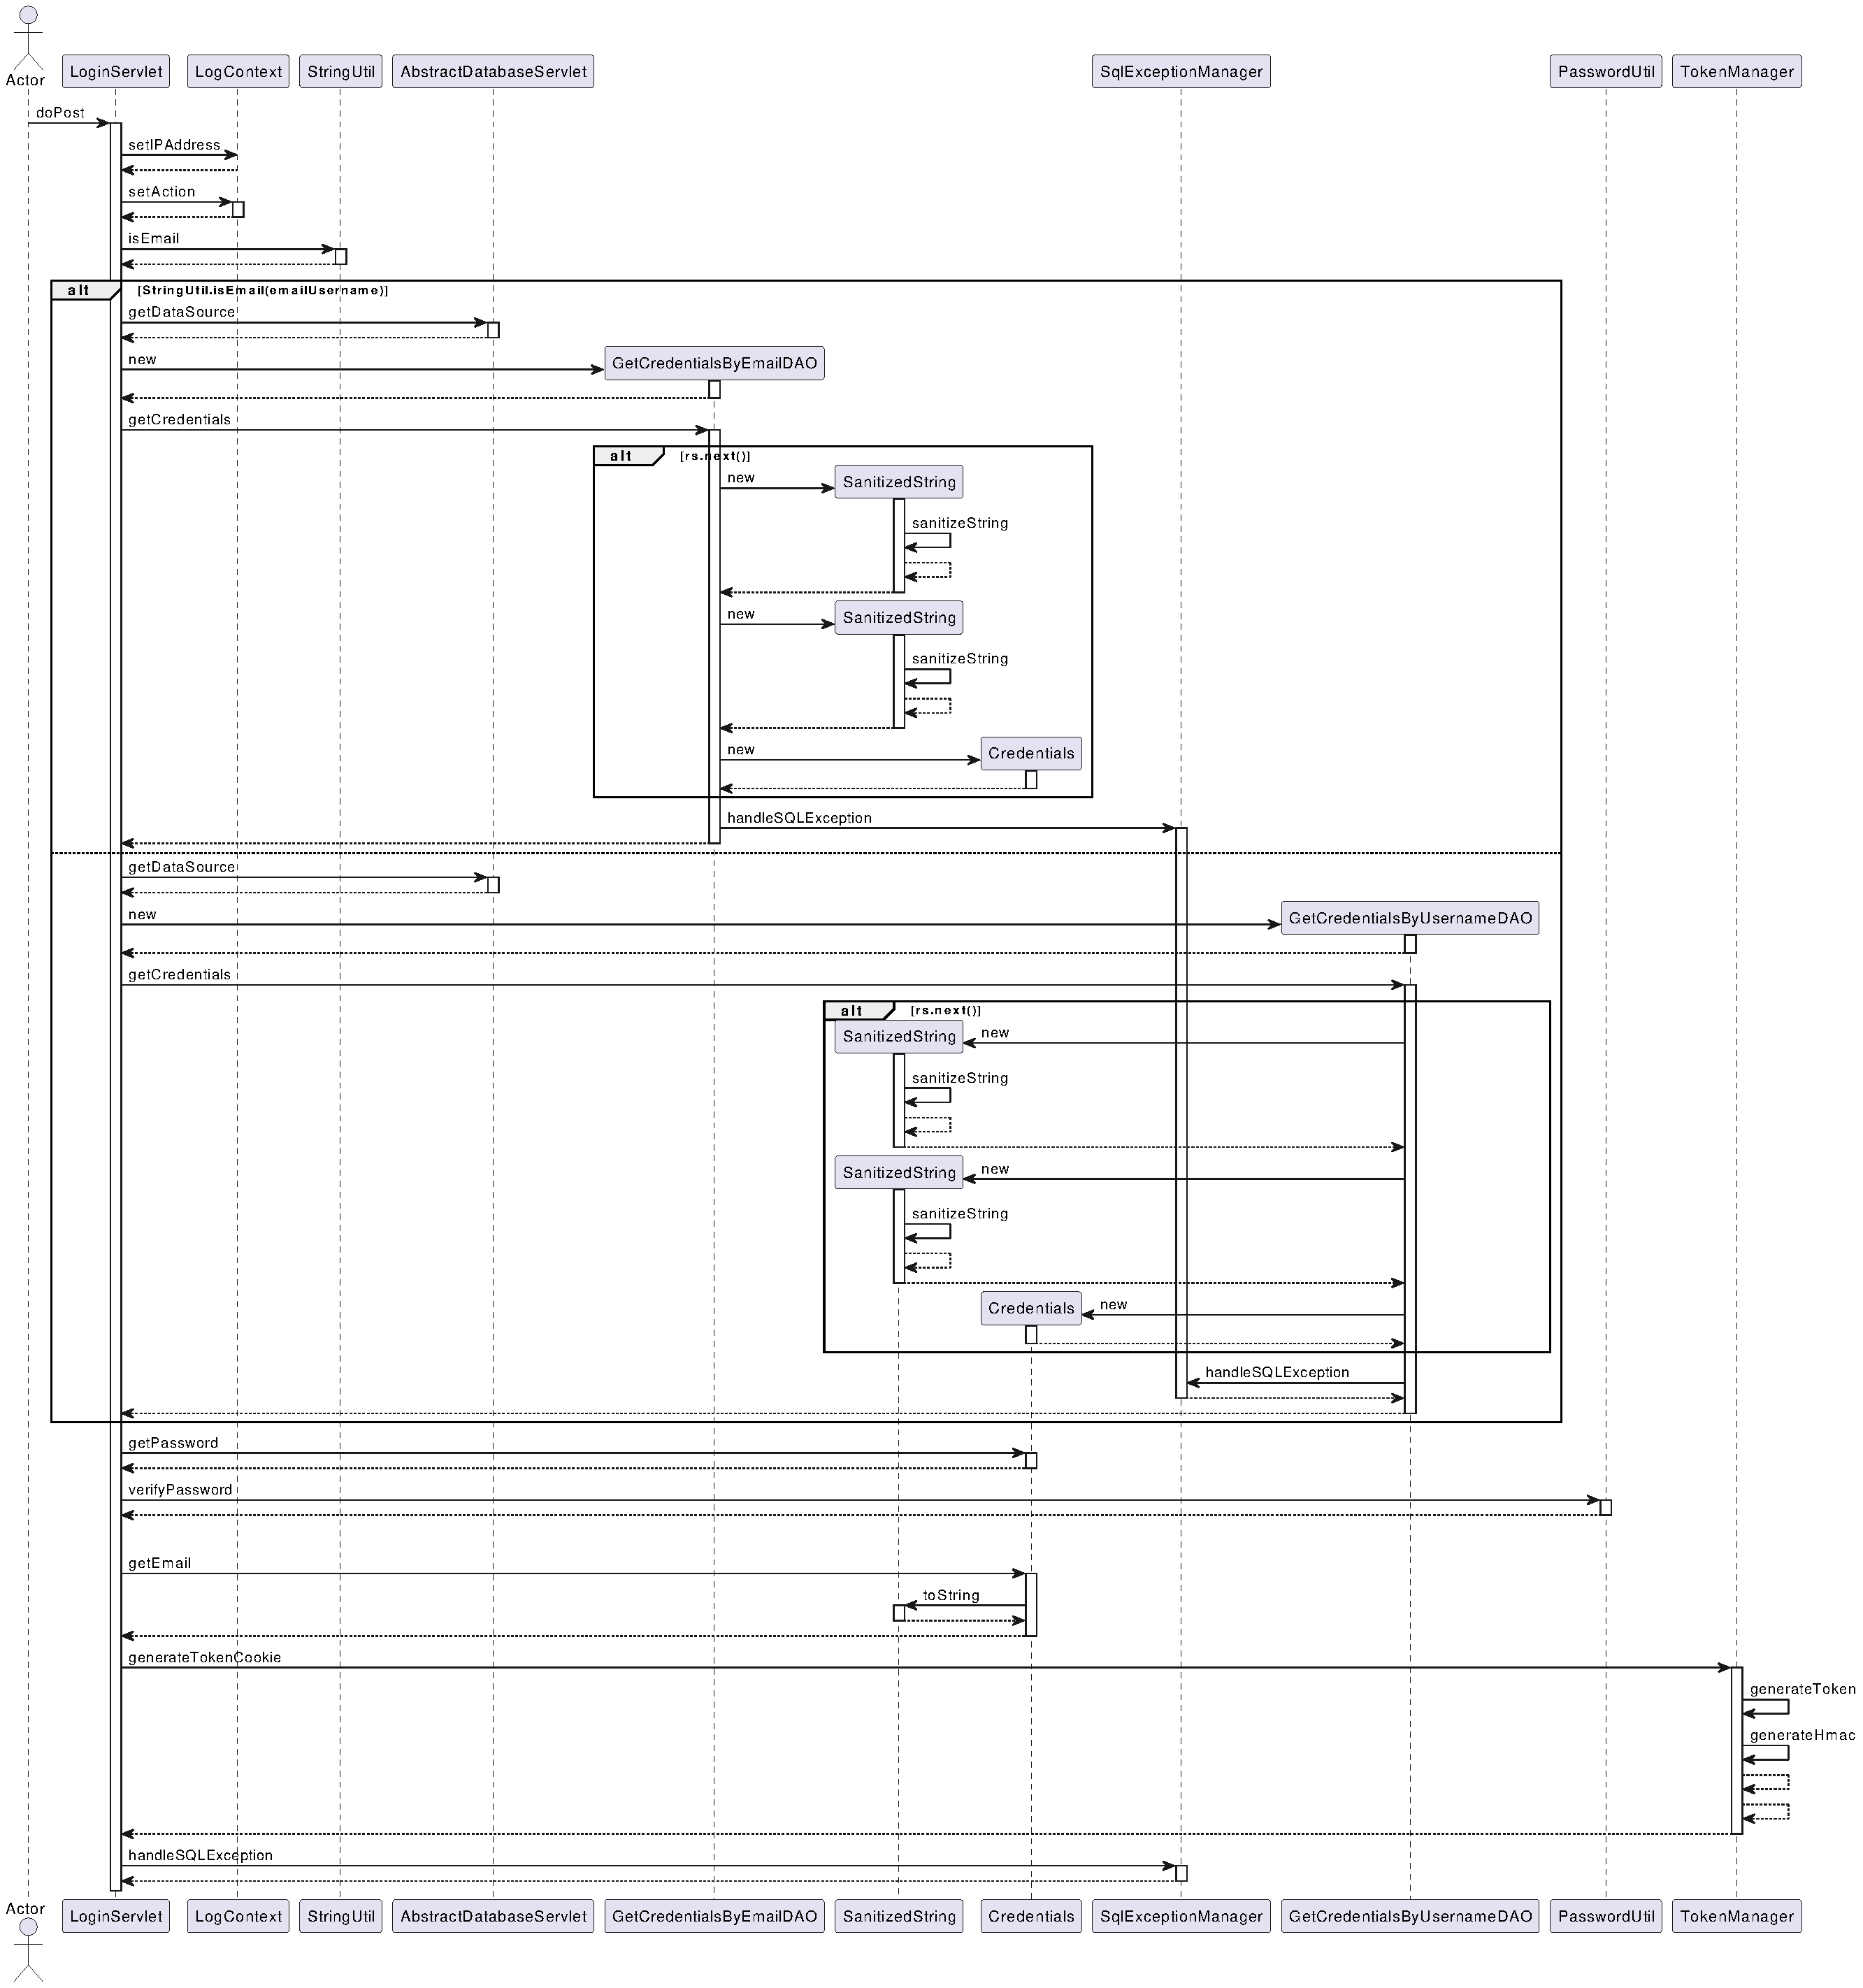
\includegraphics[width=\textwidth]{images/sequence_diagrams/Login.pdf}
    \caption{Login Sequence Diagram}
\end{figure}

The sequence diagram illustrates the entire login operation, beginning when the end user issues an HTTP POST to the LoginServlet, supplying their identifier (either an email address or a username) and password. As soon as LoginServlet.doPost(request, response) executes, it records the client’s IP address and the “login” action via calls to LogContext.setIPAddress(...) and LogContext.setAction(...). Next, the servlet must decide whether the supplied identifier is an email or simply a username; it does so by invoking StringUtil.isEmail(identifier).

If the identifier is recognized as an email, the servlet retrieves a JDBC DataSource from its superclass AbstractDatabaseServlet and uses it to instantiate GetCredentialsByEmailDAO. It then calls getCredentials(email) on that DAO. Inside the DAO, a parameterized SQL query is executed, and—if the result set yields a row—the code wraps each raw string column (for example, the email and the stored password hash) in a SanitizedString by calling its sanitizeString(...) method. A new Credentials object is constructed from these sanitized values and returned to the servlet. Any SQLException thrown during this process is caught and forwarded to SQLExceptionManager.handleSQLException(...), which logs the error and aborts the normal login flow.

In the alternative branch—when the identifier is not an email—the servlet follows the same pattern but uses GetCredentialsByUsernameDAO instead. It again fetches the DataSource, instantiates the username‐based DAO, executes its getCredentials(username) method, sanitizes the result set columns, constructs a Credentials object, and handles any SQL errors via the same exception manager.

Once LoginServlet has obtained the Credentials object (regardless of which DAO was used), it retrieves the stored password hash and calls PasswordUtil.verifyPassword(submittedPassword, storedHash). If verification fails, the servlet forwards back to login.jsp and displays an appropriate error message. If verification succeeds, the servlet obtains the canonical email string by calling credentials.getEmail().toString() and proceeds to session establishment. It delegates to TokenManager.generateTokenCookie(email), which internally invokes generateToken(email) to produce the token payload and generateHmac(token) to sign it; the result is encapsulated in a cookie that is added to the HttpServletResponse. Finally, the servlet returns the post‑login page—often the user’s home or dashboard—back to the actor. Throughout the diagram, any unhandled database error bubbles up to the SQLExceptionManager, ensuring that server‑side problems are centrally logged and an error page is shown instead of a successful login.


%%%%%%%%%%%%%%%%%%%%%%%%%%%%%%%%%%%%%%%%%%%%%%%
\subsubsection{Delete Event}
\begin{figure}[H]
    \centering
    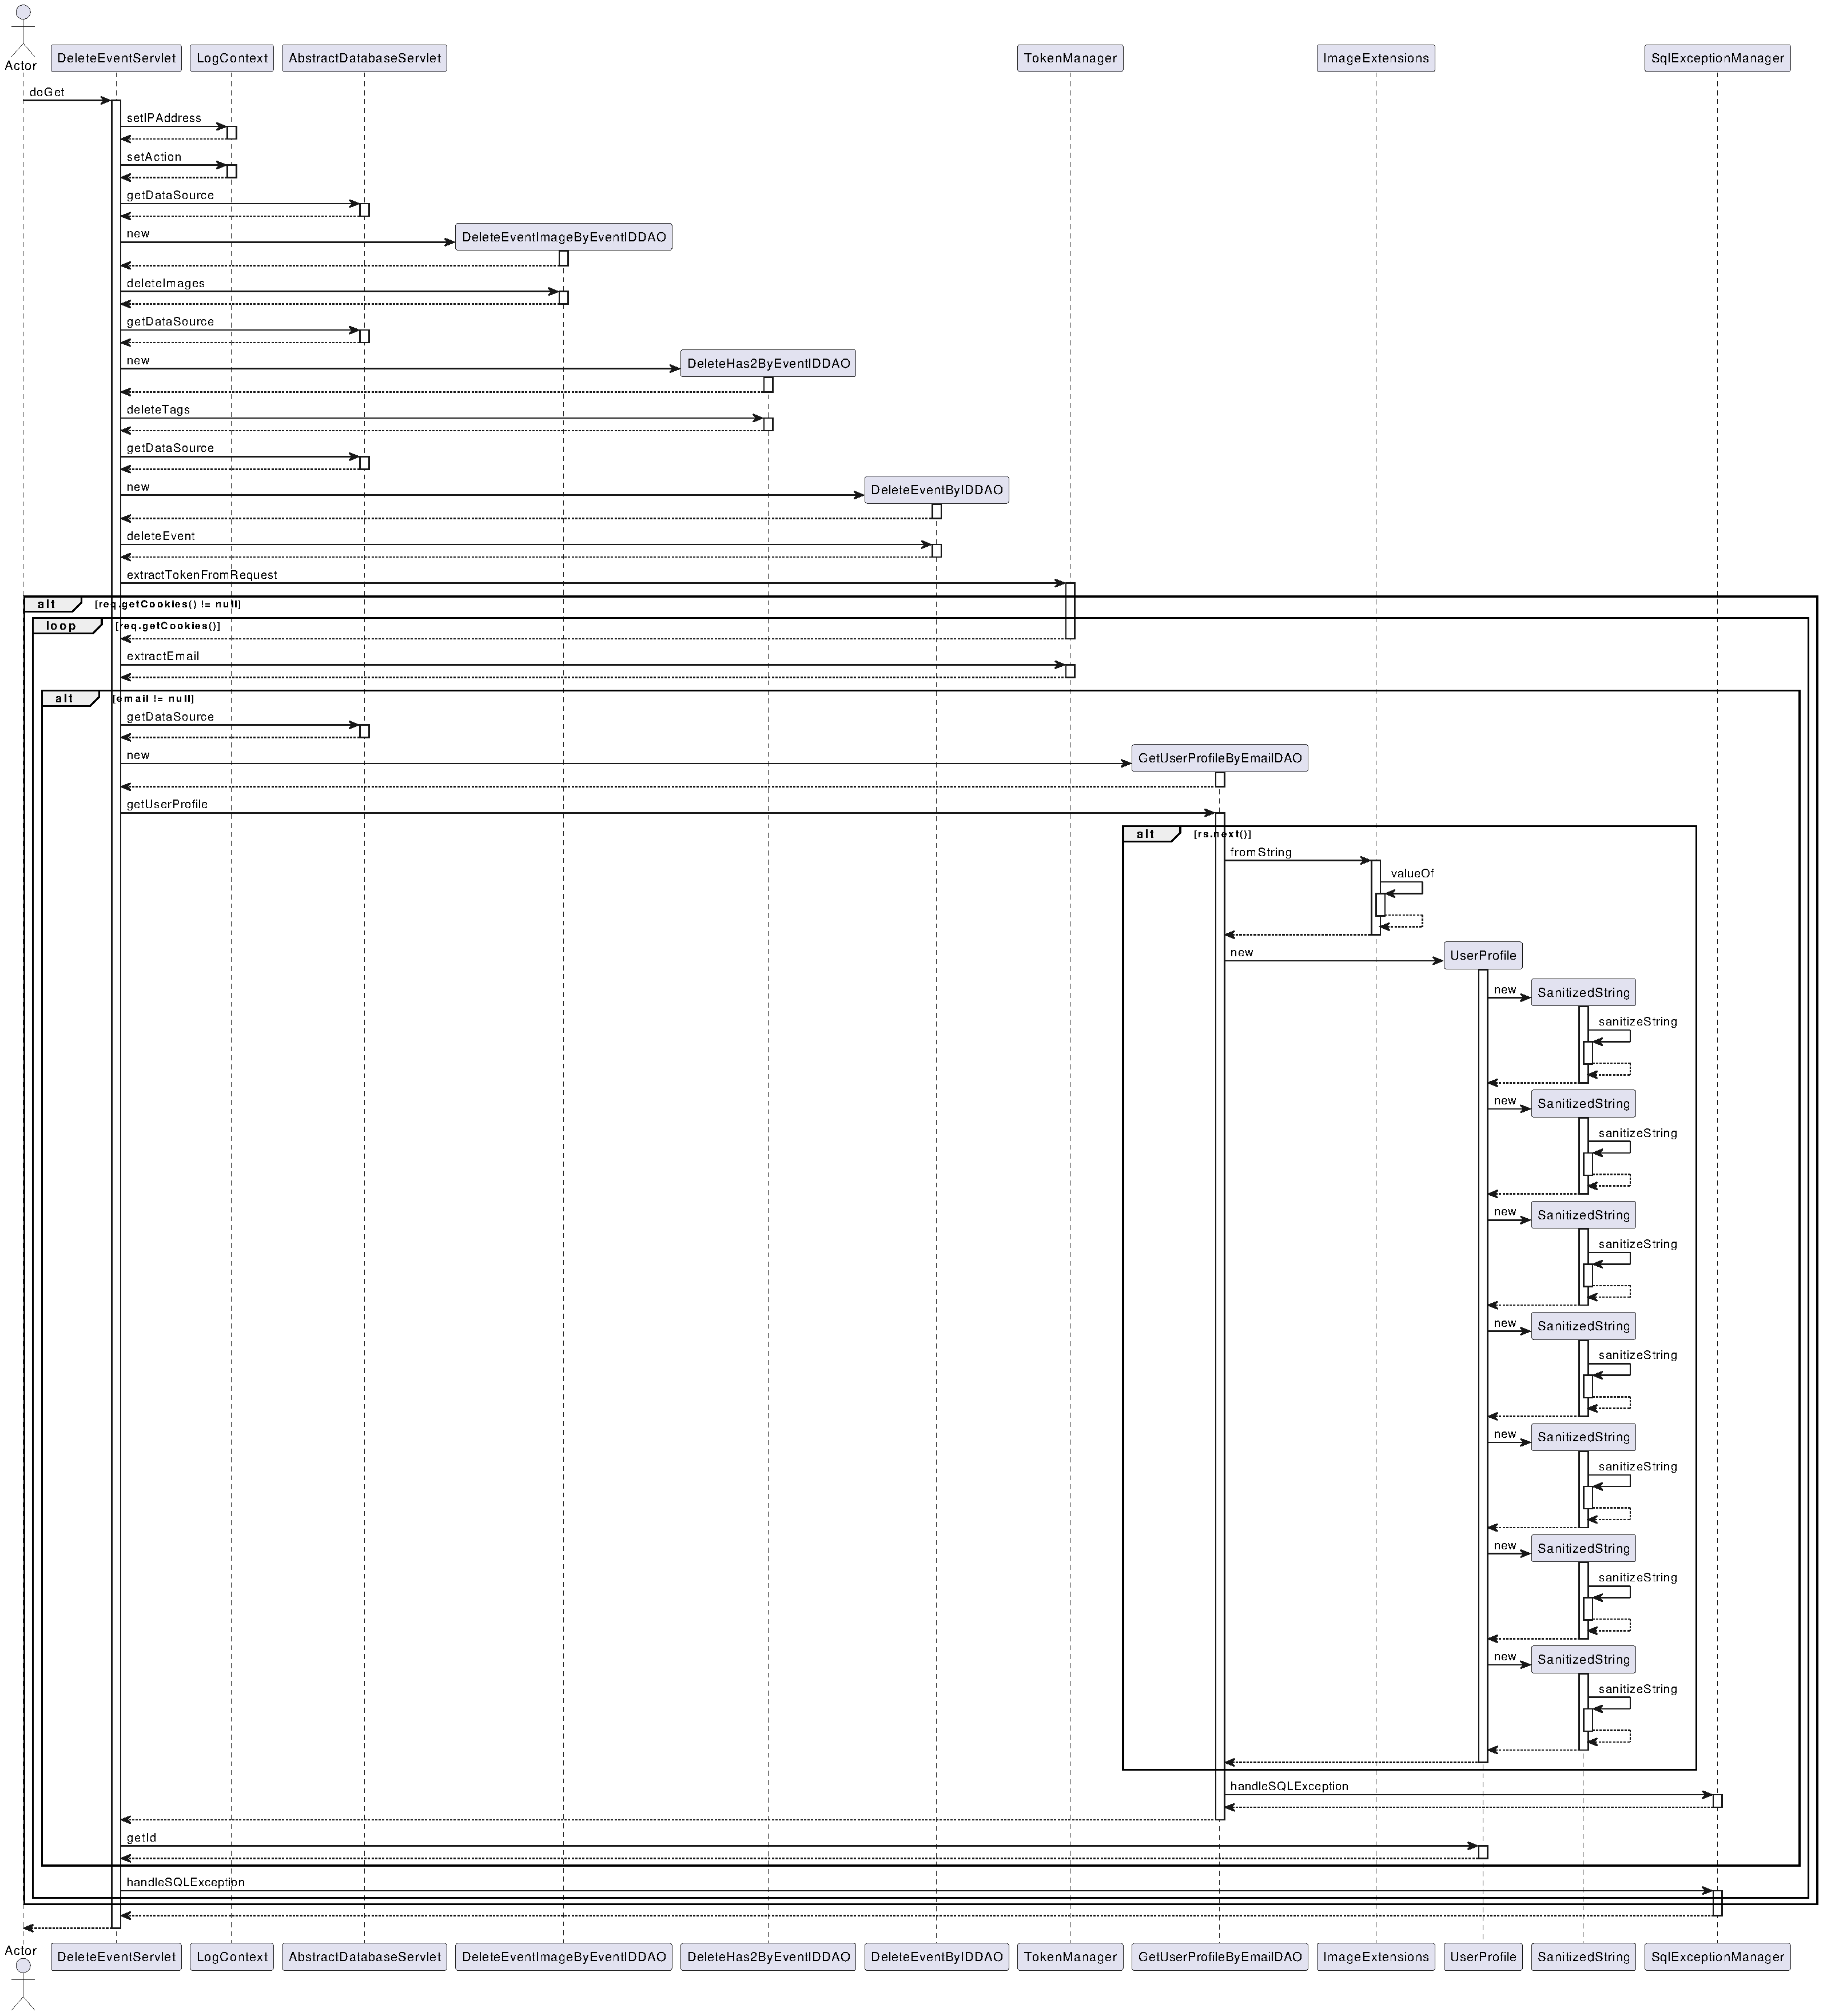
\includegraphics[width=\textwidth]{images/sequence_diagrams/DeleteEvent.pdf}
    \caption{Delete Event Sequence Diagram}
\end{figure}

Here we report the sequence diagram for the delete‑event operation. The actor initiates a GET request to the web server at the endpoint handled by DeleteEventServlet, supplying the identifier of the event to be removed. As soon as the request arrives, DeleteEventServlet invokes the LogContext component to record the client’s IP address and the “delete event” action in the application logs. Leveraging the database connectivity provided by its superclass AbstractDatabaseServlet, the servlet then obtains a DataSource and constructs a DeleteEventImageByEventIDDAO, calling its deleteImages method to purge all image records tied to that event. In the same fashion, it acquires a fresh DataSource, instantiates DeleteHas2ByEventIDDAO, and executes deleteTags to remove any tag associations. Finally, a third retrieval of the DataSource is used to create DeleteEventByIDDAO, whose deleteEvent method eliminates the event entry itself from the database. Throughout these DAO operations, any SQL-related errors are intercepted and propagated to SqlExceptionManager for consistent error handling and messaging.

Once the database deletions complete, DeleteEventServlet turns to authentication and user context restoration. It calls TokenManager.extractTokenFromRequest, iterating over cookies in the HTTP request to locate the authentication token. If a token—and thus an email—is successfully extracted, the servlet again uses getDataSource to spawn a GetUserProfileByEmailDAO, invoking getUserProfile to fetch the user’s profile data from the database. When the result set yields a record, the DAO employs SanitizedString repeatedly to cleanse each field (such as name, email, role) before assembling a UserProfile object. Any exceptions encountered during token extraction or profile lookup are funneled through SqlExceptionManager.handleSQLException to ensure graceful recovery. Finally, the servlet retrieves the user’s ID from the UserProfile, handles any remaining exceptions, and forwards a confirmation or redirect response—typically back to the event list page—so the actor sees that the deletion has been completed successfully.


%%%%%%%%%%%%%%%%%%%%%%%%%%%%%%%%%%%%%%%%%%%%%%%
\subsubsection{Follows}
\begin{figure}[H]
    \centering
    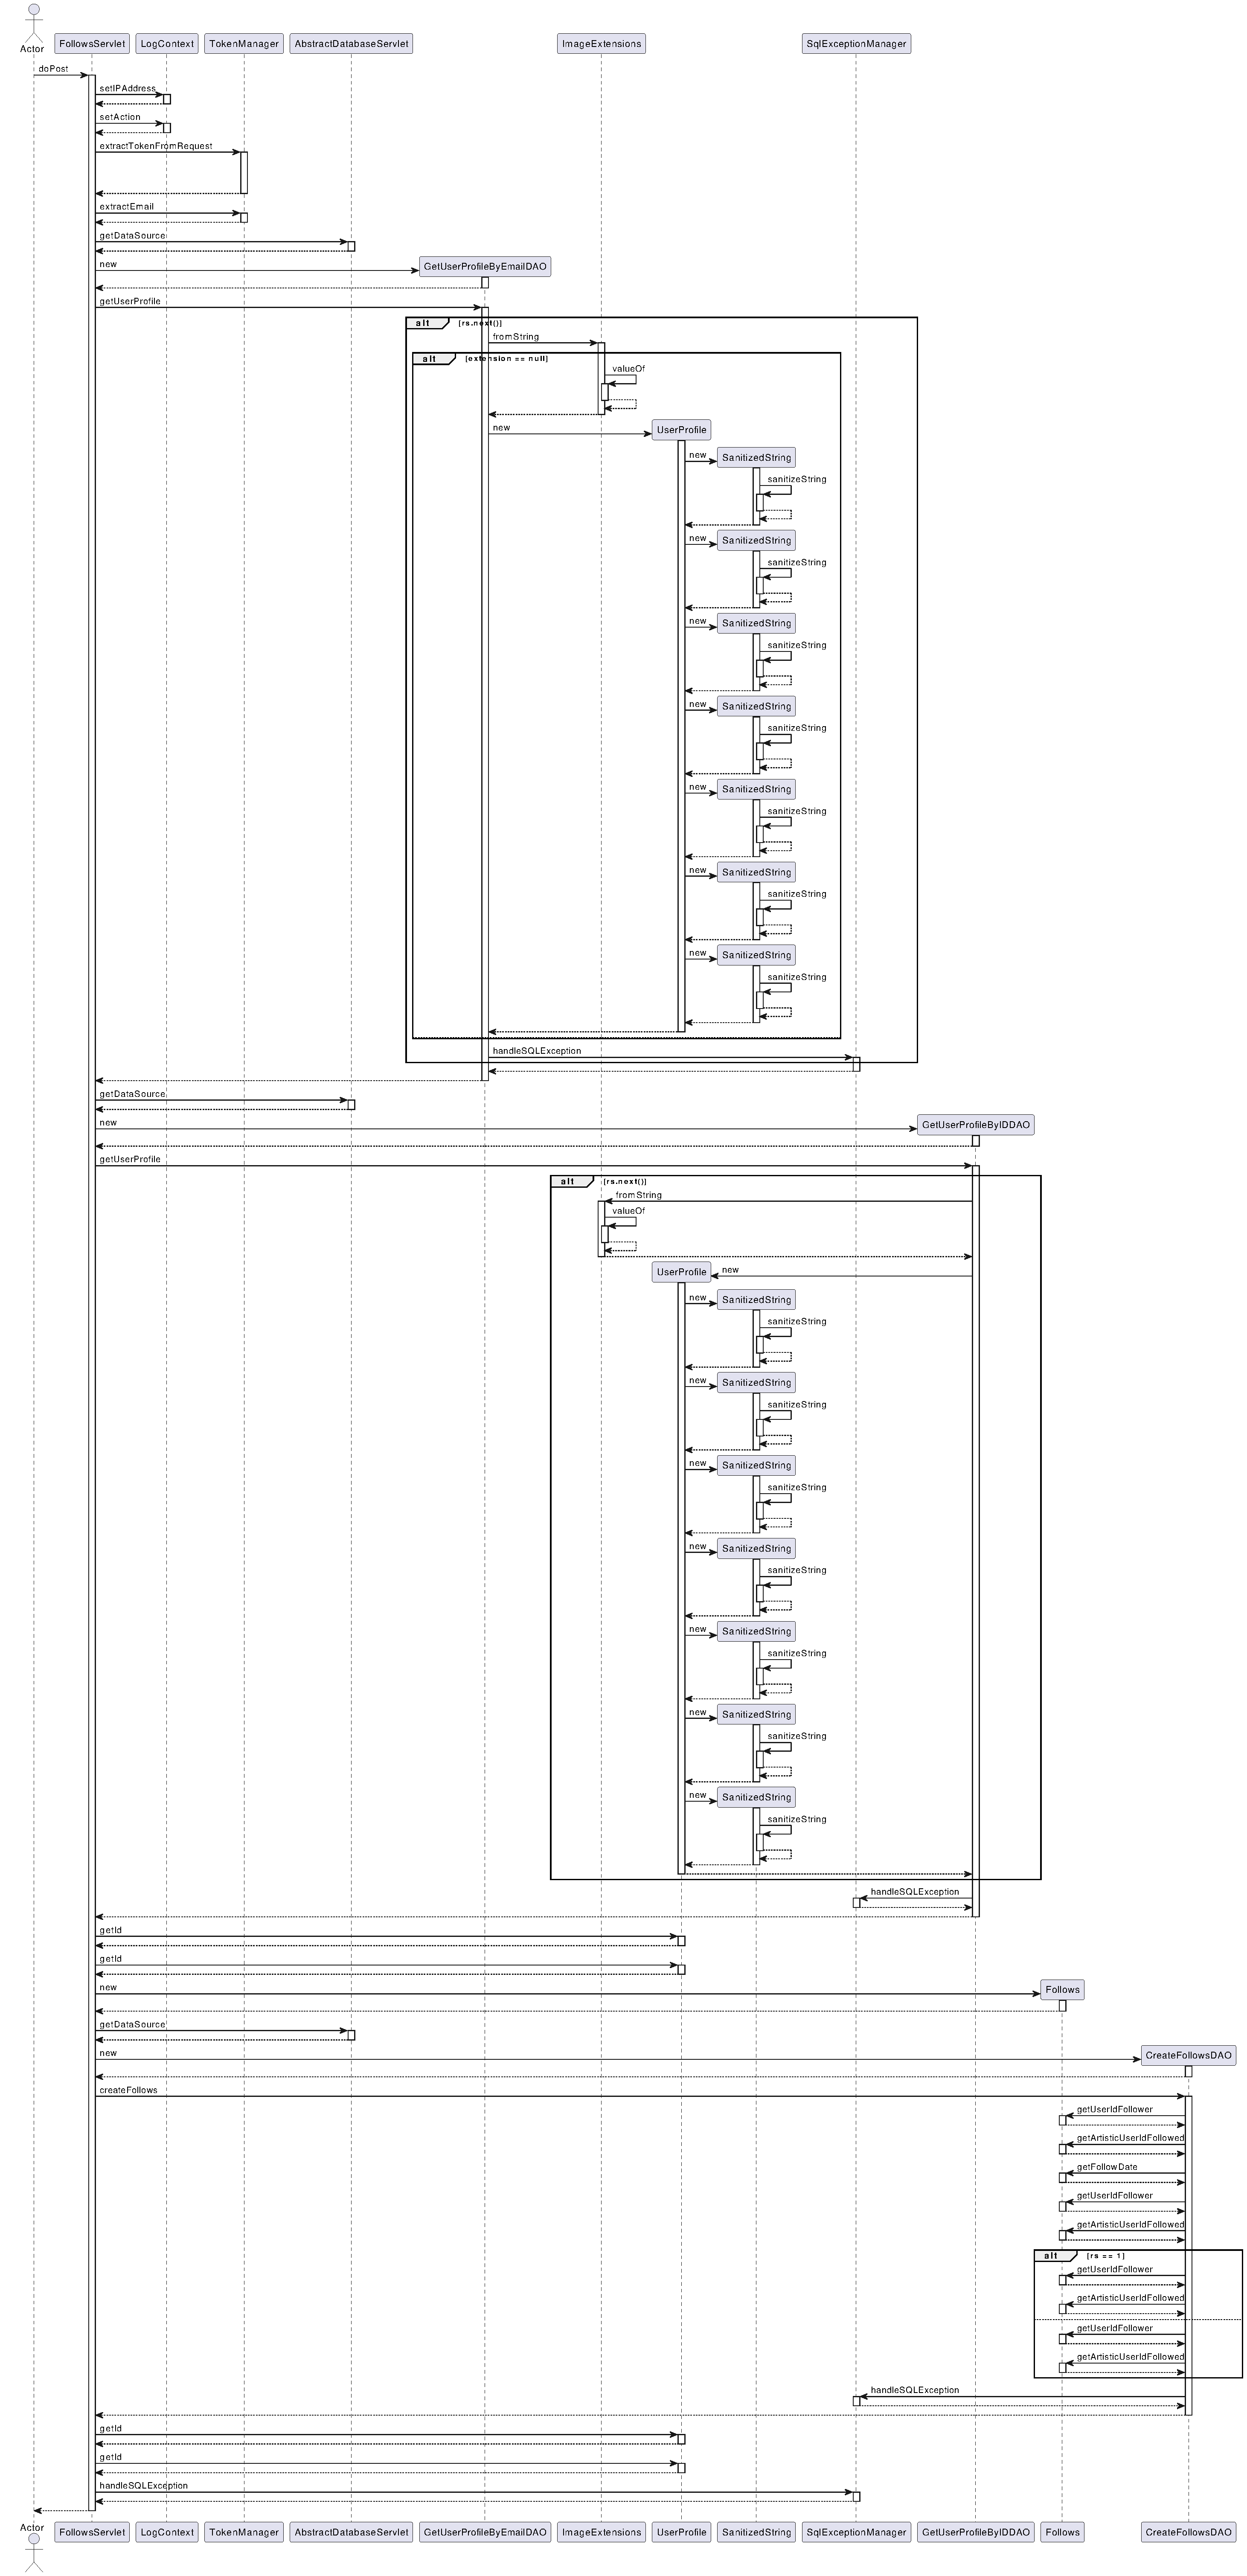
\includegraphics[width=0.7\textwidth]{images/sequence_diagrams/Follows.pdf}
    \caption{Follows Sequence Diagram}
\end{figure}

Here we report the sequence diagram for the “follow” operation. The actor issues a POST request to the web server, invoking the FollowsServlet via its doPost method and supplying the identifier of the user to be followed. Immediately, LogContext is called to record the client’s IP address and the “follow” action in the application logs. Next, FollowsServlet leverages its inheritance from AbstractDatabaseServlet to obtain a DataSource and instantiates TokenManager, which scans the HTTP request’s cookies to extract the authentication token and, in turn, the actor’s email. Using that email, the servlet creates a GetUserProfileByEmailDAO and calls getUserProfile to retrieve the actor’s profile from the database. If a result is found, each field (name, email, role, etc.) is passed through SanitizedString to ensure safe input before a UserProfile object is built; any SQL exceptions along the way are funneled through SqlExceptionManager for uniform handling.

With the actor’s UserProfile in hand, FollowsServlet again calls getDataSource to instantiate GetUserProfileByIDDAO, this time passing the target user’s ID to fetch their profile. As before, the DAO sanitizes each returned field and handles exceptions via SqlExceptionManager. Once both profiles are available, the servlet extracts the follower’s ID and the followed user’s ID, and constructs a domain object Follows—populating it with userIdFollower, artisticUserIdFollowed, and the current date. A fresh DataSource is then used to create a CreateFollowsDAO, whose createFollows method inserts the new follow relationship into the database (returning a row‑count confirmation). Any errors during insertion are caught by SqlExceptionManager, and upon success the servlet forwards a confirmation response—typically redirecting the actor back to the followed user’s profile or the main feed so they see the updated state of their follows.